\section*{3. Tableau des tâches BDP}

\Large{À chaque tâche correspond une lettre :\\ }

\begin{itemize}
\item "\textcolor{red}{R}" : la Partie à qui est affectée la réalisation de la tâche.
\item "\textcolor{red}{P}" : la Partie qui doit assister l’autre Partie dans la réalisation de sa tâche. Lorsque cette tâche est attribuée au Client, il appartient au Client de transmettre au Prestataire les éléments nécessaires à la réalisation de la tâche considérée. Lorsque cette tâche est attribuée au Prestataire, il appartient au Prestataire de réaliser un transfert de compétence au bénéfice du Client.
\item "\textcolor{red}{V}" : la Partie qui doit procéder au contrôle des résultats des tâches.\\
\end{itemize}

\begin{figure}[h]
\centering
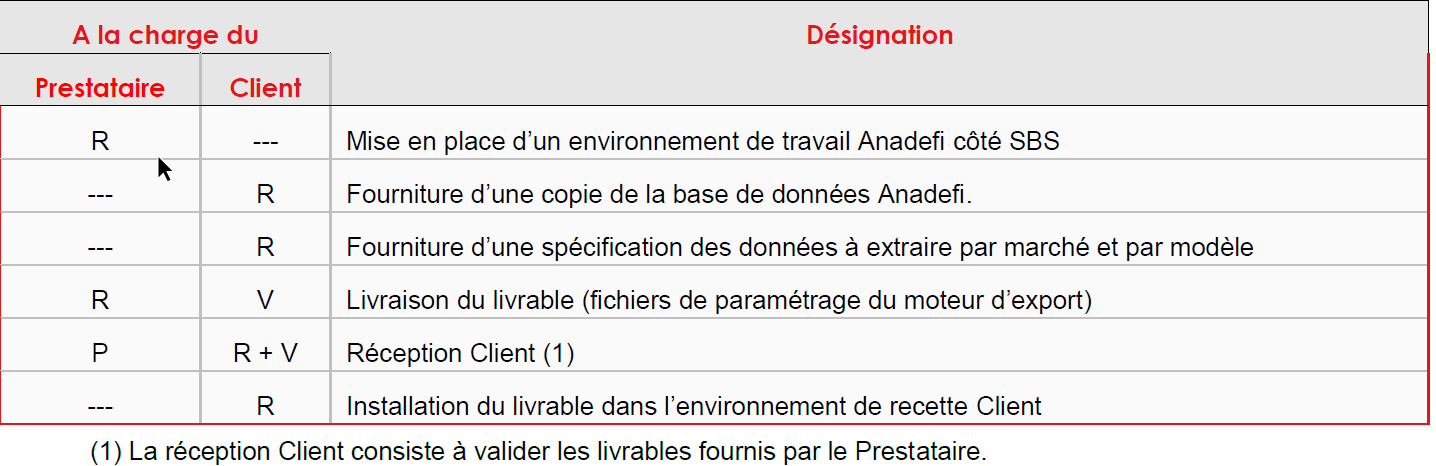
\includegraphics[scale=0.6]{resources/tachesBDP.png}
\caption{Tableau des tâches}
\label{tbl BDP}
\end{figure}